\usepackage{tikz}
\usetikzlibrary{positioning, arrows.meta, fit, backgrounds}

\begin{figure}[!htbp]
  \centering
  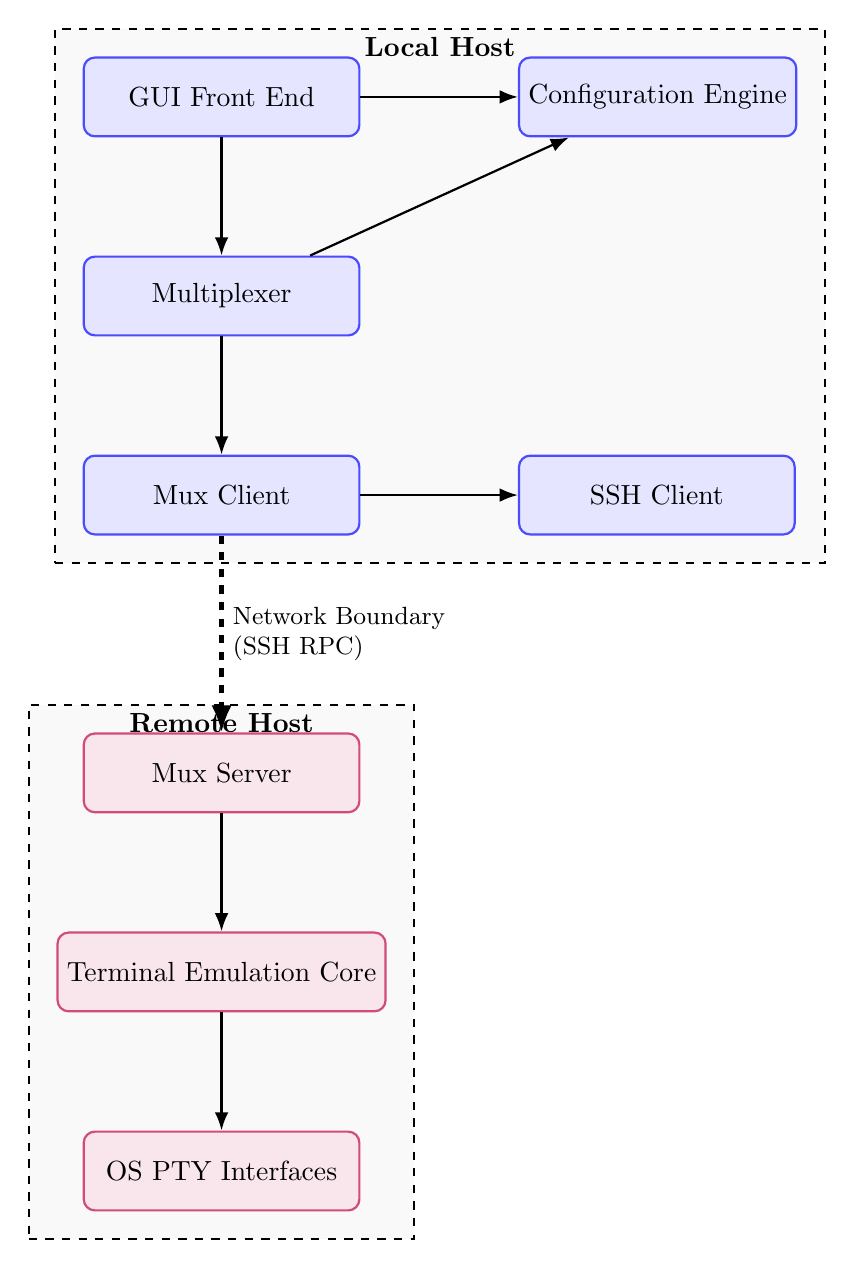
\begin{tikzpicture}[
      node distance=1.5cm and 2cm,
      box/.style={draw, thick, rounded corners, minimum width=3.5cm, minimum height=1cm, align=center},
      local/.style={box, fill=blue!10, draw=blue!70},
      remote/.style={box, fill=purple!10, draw=purple!70},
      arrow/.style={-Latex, thick},
      boundary/.style={draw, dashed, thick, inner sep=10pt}
    ]

    % Local Host Subsystems
    \node[local] (gui) {GUI Front End};
    \node[local, right=of gui] (config) {Configuration Engine};
    \node[local, below=of gui] (mux) {Multiplexer};
    \node[local, below=of mux] (muxclient) {Mux Client};
    \node[local, right=of muxclient] (ssh) {SSH Client};

    % Local Host Dependencies
    \draw[arrow] (gui) -- (mux);
    \draw[arrow] (gui) -- (config);
    \draw[arrow] (mux) -- (config);
    \draw[arrow] (mux) -- (muxclient);
    \draw[arrow] (muxclient) -- (ssh);

    % Local Host Background Boundary
    \begin{scope}[on background layer]
      \node[boundary, fit=(gui)(config)(muxclient)(ssh), fill=gray!5, label={[anchor=north, font=\bfseries]above:Local Host}] (localhost) {};
    \end{scope}

    % Remote Host Subsystems
    \node[remote, below=2.5cm of muxclient] (muxserver) {Mux Server};
    \node[remote, below=of muxserver] (term) {Terminal Emulation Core};
    \node[remote, below=of term] (pty) {OS PTY Interfaces};

    % Remote Host Dependencies
    \draw[arrow] (muxserver) -- (term);
    \draw[arrow] (term) -- (pty);

    % Remote Host Background Boundary
    \begin{scope}[on background layer]
      \node[boundary, fit=(muxserver)(term)(pty), fill=gray!5, label={[anchor=north, font=\bfseries]above:Remote Host}] (remotehost) {};
    \end{scope}

    % Network Boundary Edge
    \draw[arrow, dashed, line width=1.5pt] (muxclient) -- node[right, font=\small, align=left] {Network Boundary \\ (SSH RPC)} (muxserver);

  \end{tikzpicture}
  \caption{Conceptual architecture mapping the subsystems of WezTerm.}
  \label{fig:architecture-subsystems}
\end{figure}